\documentclass{beamer}

\usepackage{lmodern}
\usepackage[utf8]{inputenc}
\usepackage{amsmath}
\usepackage{siunitx}
\usepackage{minted}
\usepackage{svg}
\usepackage{ragged2e}
\newcommand{\jindent}{\justifying\setlength{\parindent}{1.5em}}
\setminted{
    fontsize=\scriptsize,
    bgcolor=white,
    frame=single,
    numbers=left,
    breaklines=true,
    breakanywhere=true
    tabsize=4}

\title{Simulador de voo}
\institute{Nisus Aerodesign}
\date{}

\begin{document}
\footnotesize
% ----------------------------------------------------------
\frame{\titlepage}
% ----------------------------------------------------------

\begin{frame}{Referências}
\begin{itemize}
    \item { Etkin, Reid - Dynamics of Flight Stability and Control }
    \item { Stevens, Lewis, Johnson - Aircraft Control and Simulation }
\end{itemize}
\end{frame}

% ----------------------------------------------------------

\begin{frame}{Eixos e notação}

    \jindent
    A Terra será tratada como plana e estacionário no espaço inercial, de modo que qualquer sistema de coordenadas na Terra é incercial. Denotamos este sistema por $F_E(O_E, x_E, y_E, z_E)$, e sua origem é posicionada arbitrariamente. O eixo $O_E z_E$ aponta verticalmente para baixo, e o eixo $O_E x_E$ é geralmente apontado para o norte ou alguma direção de referência. Este sistema é frequentemente denominado \textit{North-East-Down} (NED).
    
    \jindent
    A velocidade do CG da aeronave relativa à $F_E$ é $\mathbf{V}^E$ e denominada \textit{groundspeed}.
    
    \jindent
    As forças aerodinâmicas não dependem da velocidade relativa à $F_E$, mas da velocidade da aeronave relativa à massa de ar (\textit{airspeed}), que difere de $\mathbf{V}^E$ por conta do vento $\mathbf{W}$. Se $\mathbf{V}$ é a velocidade do $CG$ relativo ao ar, então

    \begin{equation*}
        \mathbf{V}^E = \mathbf{V} + \mathbf{W}        
    \end{equation*}
    
\end{frame}

% ----------------------------------------------------------

\begin{frame}{Eixos e notação}

    \jindent
    Um segundo sistema de referência $F_B$ (\textit{body axes}), fixo à aeronave e origem $C$ no $CG$, será necessário para o desenvolvimento das equações do movimento.
    
\end{frame}

% ----------------------------------------------------------

\begin{frame}{Eixos e notação}
    \begin{figure}
        \centering
        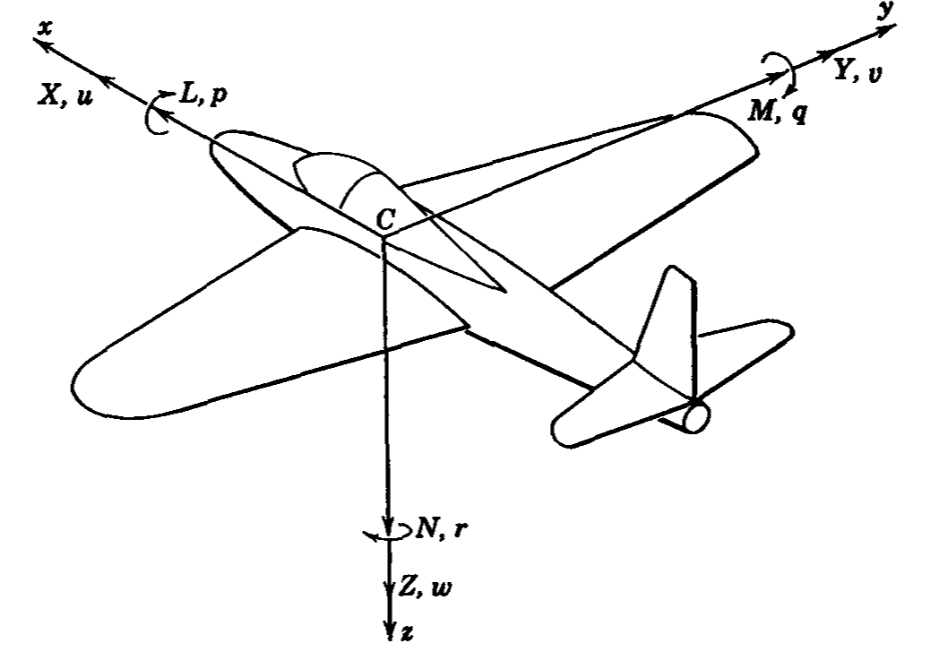
\includegraphics[width=0.7\textwidth]{bodyaxes.png}
        \caption{Notação do sistema de referências do corpo. l = momento de rolagem, m = momento de arfagem, n = momento de guinada, p = taxa de rolagem, q = taxa de arfagem, r = taxa de guinada. [X, Y, Z] = componentes da força aerodinâmica resultante. [u, v, w] = componentes da velocidade do centro de massa da aeronave relativa à atmosfera.}
    \end{figure}
\end{frame}

% ----------------------------------------------------------

\begin{frame}{Equações do movimento}

    \jindent
    É necessário determinar as equações de movimento translacional e rotacional de um corpo com 6 graus de liberdade. Os dois conjuntos de equação são

    \begin{align*}
        \mathbf{f}_E &= m \dot{\mathbf{V}}_E^E \\
        \mathbf{G}_E &= \dot{\mathbf{h}}_E 
    \end{align*}

    \justifying
    em que $\mathbf{f}_E$ é a força resultante, $\mathbf{G}_E$ é o momento resultante, $m$ e $\mathbf{h}_E$ são respectivamente a massa e o momento angular da aeronave. $\mathbf{V}_E^E$ é a velocidade relativa à Terra (superscrito), expressa no referencal da Terra (subscrito),

    \begin{equation*}
        \mathbf{V}_E^E = \begin{bmatrix} \dot x_E \\ \dot y_E \\ \dot z_E \end{bmatrix}
    \end{equation*}

\end{frame}

% ----------------------------------------------------------

\begin{frame}{Equações de navegação}
    \jindent
    Para rastrear a trajetória de voo relativo à Terra ($F_E$), é necessário obter as componentes da velocidade transformando o vetor $\mathbf{V}_B^E$ em $\mathbf{V}_E^E$, por meio da transformação

    \begin{equation*}
        \mathbf{V}_E^E = \mathbf L_{EB}\mathbf{V}_B^E
    \end{equation*}

    \justifying
    em que $\mathbf L_{EB}$ é a matriz de cossenos diretores que corresponde à reversão de rotação que se realiza para orientar a aeronave com base nos ângulos de Euler.

    \begin{equation*}
    \mathbf L_{EB} =
        \begin{bmatrix}
        \cos\theta \cos\psi &
        \sin\phi \sin\theta \cos\psi - \cos\phi \sin\psi &
        \cos\phi \sin\theta \cos\psi + \sin\phi \sin\psi \\
        
        \cos\theta \sin\psi &
        \sin\phi \sin\theta \sin\psi + \cos\phi \cos\psi &
        \cos\phi \sin\theta \sin\psi - \sin\phi \cos\psi \\
        
        -\sin\theta &
        \sin\phi \cos\theta &
        \cos\phi \cos\theta
        \end{bmatrix}
    \end{equation*}

    \jindent
    Este sistema são as equações de navegação do corpo (lembre-se que  $\mathbf{V}_E^E = \begin{bmatrix} \dot x_E & \dot y_E &\dot z_E \end{bmatrix}^T$)

    
\end{frame}

% ----------------------------------------------------------

\begin{frame}{Equações do movimento}
    \jindent
    Para determinar o momento ângular, seja a velocidade ângular da aeronave
    
    \begin{equation*}
        \boldsymbol{\omega}_B =
            \begin{bmatrix}
            p \\ q \\ r 
            \end{bmatrix}
    \end{equation*}

    \justifying
    e a matriz de inércia
    
    \begin{equation*}
        \mathbf I_B =
        \begin{bmatrix}
        I_x   & -I_{xy} & -I_{xz} \\
        -I_{yx} & I_y   & -I_{yz} \\
        -I_{zx} & -I_{zy} & I_z
        \end{bmatrix}
    \end{equation*}

    \justifying
    temos que

    \begin{equation*}
        \mathbf{h}_B = \mathbf{I}_B \boldsymbol{\omega}_B
    \end{equation*}
    
\end{frame}


% ----------------------------------------------------------

\begin{frame}{Equações do movimento}
    \jindent
    A variação dos ângulos de Euler são obtidas  por

    \begin{equation*}
        \begin{bmatrix}
            p \\q \\r
        \end{bmatrix}
            = \mathbf R
        \begin{bmatrix}
            \dot{\phi} \\
            \dot{\theta} \\
            \dot{\psi}
        \end{bmatrix}
    \end{equation*}

    \justifying
    em que

    \begin{equation*}
        \mathbf R =
        \begin{bmatrix}
            1 & 0 & -\sin\theta \\
            0 & \cos\phi & \sin\phi \cos\theta \\
            0 & -\sin\phi & \cos\phi \cos\theta
        \end{bmatrix}
    \end{equation*}

    \jindent
    Invertendo, obtém-se as taxas dos ângulos de Euler

    \begin{equation*}
        \begin{bmatrix}
            \dot{\phi} \\
            \dot{\theta} \\
            \dot{\psi}
        \end{bmatrix}
         = \mathbf T
        \begin{bmatrix}
            p \\q \\r
        \end{bmatrix}
    \end{equation*}

    \justifying
    onde

    \begin{equation*}
        \mathbf T =
        \begin{bmatrix}
            1 & \sin\phi \tan\theta & \cos\phi \tan\theta \\
            0 & \cos\phi & -\sin\phi \\
            0 & \sin\phi \sec\theta & \cos\phi \sec\theta
        \end{bmatrix}
    \end{equation*}

\end{frame}

% ----------------------------------------------------------

\begin{frame}{Equações do movimento de Euler}
    Finalmente, a equação da força pode ser expressa nos componentes de $F_B$

    \begin{gather*}
        \mathbf f_E = m \dot{\mathbf V}_E^E \\
        \mathbf L_{EB} \mathbf f_B = m (\dot{\mathbf L}_{EB} \mathbf V_B^E + \mathbf L_{EB} \dot{\mathbf V}_B^E)\\
        \mathbf L_{EB} \mathbf f_B = m \mathbf L_{EB} ( \tilde{\boldsymbol{\omega}}_B \mathbf V_B^E + \dot{\mathbf V}_B^E )\\
        \mathbf f_B = m (\dot{\mathbf V}_B^E + \tilde{\boldsymbol{\omega}}_B \mathbf V_B^E)
    \end{gather*}

    \justifying
    onde

    \begin{equation*}
        \tilde{\boldsymbol{\omega}}_B =
        \begin{bmatrix}
        0 & -r & q \\
        r & 0 & -p \\
        -q & p & 0
        \end{bmatrix}
    \end{equation*}

    \jindent
    O vetor $\mathbf f_B$ é a soma da gravidade $\mathbf g$ (sempre será constante) com a força aerodinâmica $\mathbf A$

    \begin{gather*}
        \mathbf A_B =
            \begin{bmatrix} X & Y & Z \end{bmatrix}^T \\
        m \mathbf g_B = m \mathbf L_{BE} \mathbf g_E = m \mathbf L_{BE}
             \begin{bmatrix} 0 & 0 & g \end{bmatrix}^T
    \end{gather*}
\end{frame}

% ----------------------------------------------------------
\begin{frame}{Equações de movimento de Euler}

    \jindent
    Finalmente, denota-se $\mathbf V_B^E = [u^E \quad v^E \quad w^E]^T$, e substituindo todas as relações anteriores, chegamos as Equações do movimento translacionais
    \begin{gather*}
    X - mg \sin \theta = m(\dot{u}^E + q w^E - r v^E) \\
    Y + mg \cos \theta \sin \phi = m(\dot{v}^E + r u^E - p w^E) \\
    Z + mg \cos \theta \cos \phi = m(w^E + p v^E - q u^E)
    \end{gather*}
    \justifying ou, isolando as derivadas da velocidade (forma que será implementada):
    \begin{gather*}
        \dot{u}^E = \frac{X}{m} - g \sin\theta - q w^E + r v^E \\
        \dot{v}^E = \frac{Y}{m} + g \cos\theta \sin\phi - r u^E + p w^E \\
        \dot{w}^E = \frac{Z}{m} + g \cos\theta \cos\phi - p v^E + q u^E
    \end{gather*}

\end{frame}


% ----------------------------------------------------------
\begin{frame}{Equações do movimento de Euler}

    \jindent
    Um procedimento similar pode ser realizado com a equação do momento angular, para obter

    \begin{equation*}
        \mathbf G_B = \dot{\mathbf h}_B + \tilde{\boldsymbol{\omega}}_B \mathbf h_B
    \end{equation*}

    \justifying e sendo $\mathbf G_B = [l \quad m \quad n]^T$, e assumindo que a aeronave é rígida ($\dot{\mathbf I}V = 0$), 
    
    \begin{gather*}
    L = I_x \dot{p} - I_{yz}(q^2 - r^2) - I_{zx}(\dot{r} + pq) - I_{xy}(\dot{q} - rp) - (I_y - I_z)qr \\
    M = I_y \dot{q} - I_{zx}(r^2 - p^2) - I_{xy}(\dot{p} + qr) - I_{yz}(\dot{r} - pq) - (I_z - I_x)rp \\
    N = I_z \dot{r} - I_{xy}(p^2 - q^2) - I_{yz}(\dot{q} + rp) - I_{zx}(\dot{p} - qr) - (I_x - I_y)pq
    \end{gather*}
        \jindent
    Uma hipótese simplificadora é a de que, se a aeronave é simétrica no plano $xz$, os produtos de inércia $I_{xy} = I_{yz} = 0$. Com isso,

    \begin{gather*}
    \dot{p} = \frac{I_{xz}(I_x - I_y + I_z)pq - \big[I_z(I_z - I_y) + I_{xz}^2\big]qr + I_z l + I_{xz} n}{I_x I_z - I_{xz}^2} \\
    \dot{q} = \frac{(I_z - I_x)rp - I_{xz}(p^2 - r^2) + M}{I_y} \\
    \dot{r} = \frac{-I_{xz}(I_x - I_y + I_z)qr + \big[I_x(I_x - I_y) + I_{xz}^2\big]pq + I_{xz} l + I_x n}{I_x I_z - I_{xz}^2}
    \end{gather*}

\end{frame}

% ----------------------------------------------------------

\begin{frame}{Variáveis de estado}
    \jindent
    Uma variável de estado é uma variável que compõe o menor conjunto de grandezas capazes de descrever completamente o estado interno de um sistema dinâmico em um instante de tempo, de modo que, conhecidas essas variáveis em $t_0$ e as entradas $u(t)$ para $t \ge t_0$, a evolução do sistema é unicamente determinada.

    \jindent
    No simulador de voo, $x_i$ são as variáveis de estado (posição, velocidade, etc) e $u_i$ serão entradas de controle (deflexão de superfícies de controle, etc), na forma geral:
    
    \begin{gather*}
        \dot{x}_1 = f_1(x_1, x_2, \dots, x_n, u_1, u_2, \dots, u_m) \\
        \dot{x}_2 = f_2(x_1, x_2, \dots, x_n, u_1, u_2, \dots, u_m) \\
        \vdots \\
        \dot{x}_n = f_n(x_1, x_2, \dots, x_n, u_1, u_2, \dots, u_m)
    \end{gather*}

    \jindent
    Essa equação pode ser escrita na forma vetorial

    \begin{equation*}
        \dot{\mathbf x} = f(\mathbf x, \mathbf u)
    \end{equation*}

    \justifying
    em que $\mathbf x$ é o vetor de estado. 
    
\end{frame}

% ----------------------------------------------------------

\begin{frame}{Variáveis de estado}
    As variáveis que compõem o vetor de estado são 12, e seus valores inicias são dados de entrada:

    \begin{itemize}
        \item Posição do CG: $x_E, y_E, z_E$
        \item Atitude: $\psi, \theta, \phi$
        \item Velocidade: $u^E, v^E, w^E$
        \item Velocidade angular: $p, q, r$
    \end{itemize}

    \jindent

\end{frame}

% ----------------------------------------------------------

\begin{frame}{Equações de estado}
    As equações de estado são as seguintes:

    \justifying \textbf{Equações de navegação}:

    \begin{gather*}
        \dot{x}_E = u^E \cos\theta \cos\psi 
                   + v^E (\sin\phi \sin\theta \cos\psi - \cos\phi \sin\psi) \\
                   \qquad + w^E (\cos\phi \sin\theta \cos\psi + \sin\phi \sin\psi) \\[6pt]
        \dot{y}_E = u^E \cos\theta \sin\psi 
                   + v^E (\sin\phi \sin\theta \sin\psi + \cos\phi \cos\psi) \\
                   \qquad + w^E (\cos\phi \sin\theta \sin\psi - \sin\phi \cos\psi) \\[6pt]
        \dot{z}_E = -u^E \sin\theta + v^E \sin\phi \cos\theta + w^E \cos\phi \cos\theta
    \end{gather*}

    \justifying \textbf{Equações cinemáticas de Euler}

    \begin{gather*}
    \dot{\phi} = p + (q \sin\phi + r \cos\phi) \tan\theta \\
    \dot{\theta} = q \cos\phi - r \sin\phi \\
    \dot{\psi} = (q \sin\phi + r \cos\phi) \sec\theta
    \end{gather*}

\end{frame}

% ----------------------------------------------------------

\begin{frame}{Equações de estado}

    \justifying \textbf{Equações do movimento de Euler (Translacionais)}

    \begin{gather*}
        \dot{u}^E = \frac{X}{m} - g \sin\theta - q w^E + r v^E \\
        \dot{v}^E = \frac{Y}{m} + g \cos\theta \sin\phi - r u^E + p w^E \\
        \dot{w}^E = \frac{Z}{m} + g \cos\theta \cos\phi - p v^E + q u^E
    \end{gather*}

    \justifying \textbf{Equações do movimento de Euler (Rotacionais)}
    
    \begin{gather*}
    \dot{p} = \frac{I_{xz}(I_x - I_y + I_z)pq - \big[I_z(I_z - I_y) + I_{xz}^2\big]qr + I_z L + I_{xz} N}{I_x I_z - I_{xz}^2} \\
    \dot{q} = \frac{(I_z - I_x)rp - I_{xz}(p^2 - r^2) + M}{I_y} \\
    \dot{r} = \frac{-I_{xz}(I_x - I_y + I_z)qr + \big[I_x(I_x - I_y) + I_{xz}^2\big]pq + I_{xz} L + I_x N}{I_x I_z - I_{xz}^2}
    \end{gather*}
\end{frame}

% ----------------------------------------------------------

\begin{frame}{Solução das equações de estado}

    \jindent
    Um método numérico é necessário para resolver as equações de estado e obter a trajetória da aeronave. Dada uma condição inicial $\mathbf x(t_0)$ e entradas $\mathbf u(t)$, deve-se calcular valores discretos sequenciais do estado

    \begin{equation*}
        \mathbf x(t_0 + k\Delta t), \quad k = 1, 2, \dots
    \end{equation*}

    \justifying
    para satisfazer

    \begin{equation*}
        \dot{\mathbf x } (t) = f(\mathbf x(t), \mathbf u(t))
    \end{equation*}

    Este é um problema de valor inicial, e o passo de tempo $\Delta t$ é um parâmetro fixo. Para resolver este problema, é possível utilizar o método de Runge-Kutta
    
\end{frame}

% ----------------------------------------------------------

\begin{frame}{Runge-Kutta}

    \jindent
    Considere a seguinte EDO,

    \begin{equation*}
        \frac{\mathrm dx}{\mathrm dt} = f(x,t)
    \end{equation*}

    \justifying 
    com condição inicial $x(t_0) = x_0$

    \jindent
    A solução discreta pode ser escrita por uma expansão em série de Taylor

    \begin{equation*}
        x(t_0 + \Delta t) = x(t_0) + \Delta t \dot{x}(t_0) + \frac{\Delta t ^2}{2!} \ddot{x}(t_0) + \dots
    \end{equation*}

    \jindent
    O método RK mais simples é o método de Euler, e consiste em truncar a série de Taylor após a primeira derivada,

    \begin{equation*}
        x_E(t_0+\Delta t) \approx x(t_0) + \Delta t f(x(t_0), t_0)
    \end{equation*}

    
\end{frame}

% ----------------------------------------------------------

\begin{frame}{Runge Kutta}
    \jindent
    No método do trapézio, uma estimatia da derivada da função no final do passo de tempo é obtida da fórmula de Euler, então, a média das derivadas no início e fim do passo de temop são usadas para um passo de tempo mais acurado:

    \begin{gather*}
        x_E(t+\Delta t) = x(t_0) + \Delta t f(x(t), t)\\
        \dot{x_E}(t+\Delta t) = f(x_E(t+\Delta t), t + \Delta t)\\
        x_T(t + \Delta t) = x(t) + \frac{\Delta t}{2} ( \dot{x}(t) + \dot{x_E}(t+\Delta t) )
    \end{gather*}

    \justifying que podem ser escritas definindo:

    \begin{gather*}
        k_1 = \Delta t f(x,t)\\
        k_2 = \Delta t f(x + k_1, t + \Delta t)\\
        x_T(t+\Delta t) = x(t) + \frac{1}{2}(k_1 + k_2)
    \end{gather*}

    Os algoritmos RK são extensões desta formulação para ordens maiores.
    
\end{frame}


% ----------------------------------------------------------

\begin{frame}{Runge Kutta}

    O Runge Kutta de 4ª ordem (RK4) possui a seguinte formulação:

    \begin{align*}
        k_1 &= \Delta t f(x,t) \\
        k_2 &= \Delta t f(x+\frac{1}{2}k_1,t+\frac{1}{2}\Delta t) \\
        k_3 &= \Delta t f(x+\frac{1}{2}k_2,t+\frac{1}{2}\Delta t) \\
        k_4 &= \Delta t f(x+k_3,t+\Delta t)  \\
        x(t+\Delta t) &= x(t) + \frac{1}{6}k_1 + \frac{1}{3}k_2 + \frac{1}{3}k_3 +\frac{1}{6}k_4
    \end{align*}
    
\end{frame}

% ----------------------------------------------------------

\begin{frame}{Modelo aerodinâmico}

    \jindent
    Nas seções anteriores, foi visto como as equações do movimento para um veículo qualquer são obtidas e resolvidas. Agora, a preocupação é modelar o comportamento aerodinâmico de uma aeronave, de modo a obter os valores das forças e momentos aerodinâmicos utilizados nas equações do movimento.

    \jindent
    As forças e momentos aerodinâmicos são produzidos pelo movimento relativo ao ar e dependem da orientação da aeronave em respeito ao escoamento. Na hipótese de um escoamento uniforme, as forças e momentos não mudam com uma rotação da aeronave na direção do escoamento, de modo que apenas dois ângulos são necessários para especificá-los. Estes são os \textit{ângulos aerodinâmicos}, o ângulo de ataque $\alpha$ e o ângulo de derrapagem $\beta$, e serão usados para obter uma transformação de eixos para um sistema de referência alinhado com o vento relativo (Eixo aerodinâmico).

    \jindent
    Visto que as forças e momentos aerodinâmicos não são calculadas no eixo aerodinâmico, é necessário obter uma rotação de eixos adequada. Note que as forças e momentos também dependem das taxas de variação angular, mas agora, estamos apenas considerando a orientação.
        
\end{frame}

% ----------------------------------------------------------

\begin{frame}{Eixo aerodinâmico}

    \jindent
    Seja o ângulo de ataque $\alpha$ definido como o ângulo entre a linha de referência da aeronave até a projeção do vento relativo no plano xz.

    \begin{figure}
        \centering
        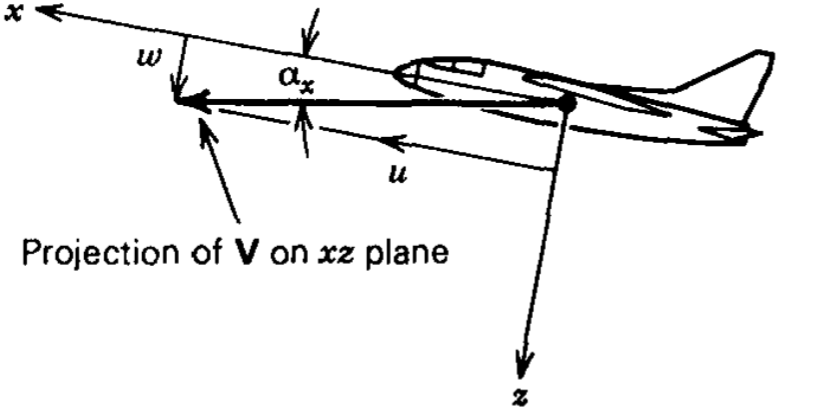
\includegraphics[width=0.3\textwidth]{alpha.png}
    \end{figure}

    \jindent
    O ângulo de derrapagem $\beta$ é medido do vento relativo à mesma projeção.

    \begin{figure}
        \centering
        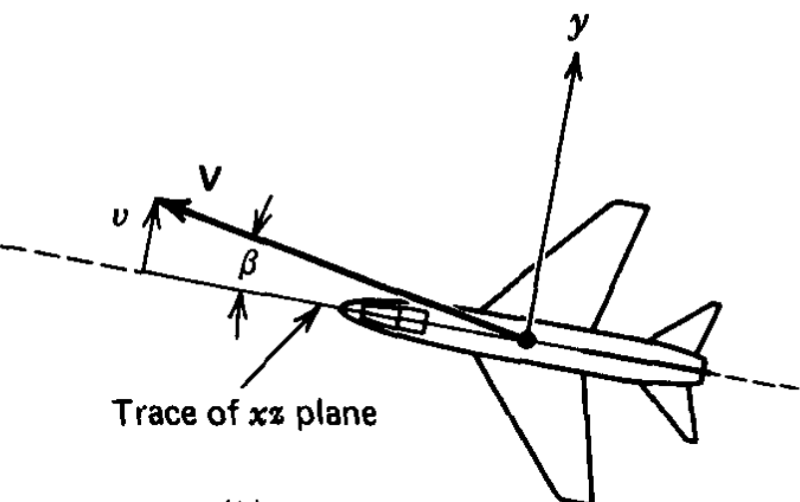
\includegraphics[width=0.3\textwidth]{beta.png}
    \end{figure}
    
\end{frame}

% ----------------------------------------------------------

\begin{frame}{Eixo aerodinâmico}

    \jindent
    O eixo obtido pela rotação do \textit{body axis} em torno de $y$ por $\alpha$ é chamado eixo de estabilidade, e é utilizado para analisar perturbações do voo em regime permanente 
    
    \jindent
    Realizando uma rotação $\beta$ no eixo $z_S$, a aeronave estará alinhada com o vento relativo. Este sistema é chamado de \textit{wind axis} (eixo aerodinâmico).
    
    \begin{figure}
        \centering
        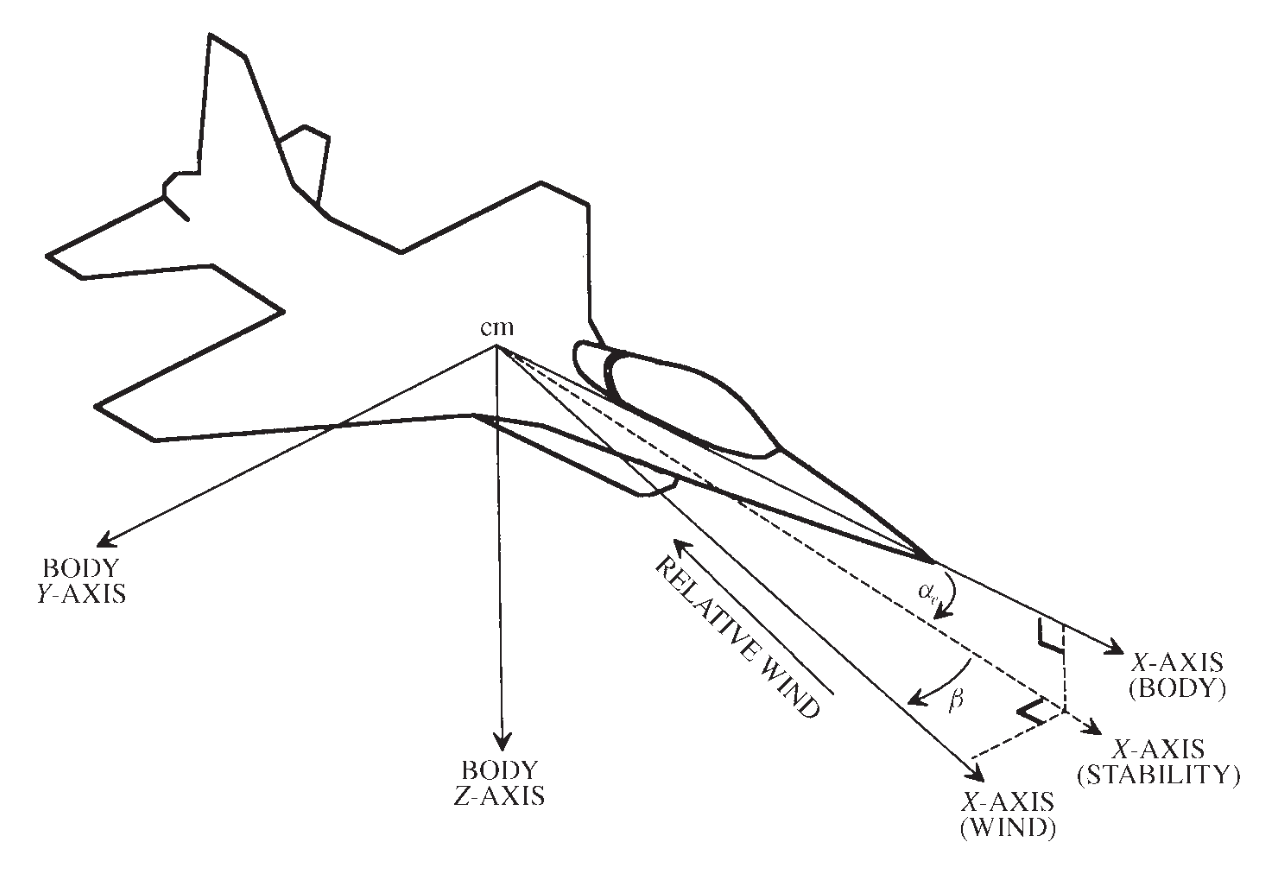
\includegraphics[width=0.5\textwidth]{windaxes.png}
    \end{figure}

    \begin{gather*}
        \alpha = \arctan \left(\frac{w_E}{u_E}\right) , \quad \quad \beta = \arcsin \left(\frac{v_E}{V}\right) \\
        V = \sqrt{u_E^2+v_E^2+w_E^2}
    \end{gather*}
    
\end{frame}

% ----------------------------------------------------------

\begin{frame}{Eixo aerodinâmico}

    A matriz de rotação responsável por trazer as componentes de um vetor na \textit{body axis} para a \textit{wind axis} é resultado de duas rotações consecutivas, como visto anteriormente:

     \begin{gather*}
        \mathbf L_{S/B} = 
        \begin{bmatrix}
            \cos\alpha & 0 & \sin\alpha \\
            0 & 1 & 0 \\
            -\sin\alpha & 0 & \cos\alpha
        \end{bmatrix} \\[10pt]
        \mathbf L_{W/B} = 
        \begin{bmatrix}
            \cos\beta & \sin\beta & 0 \\
            -\sin\beta & \cos\beta & 0 \\
            0 & 0 & 1
        \end{bmatrix}
    \end{gather*}

    \justifying
    que resulta na trasnformação direta do \textit{body axis} para a \textit{wind axis}:

    \begin{gather*}
        \mathbf{L}_{W/B} = 
        \begin{bmatrix}
        \cos\alpha \cos\beta & \sin\beta & \sin\alpha \cos\beta \\
        -\cos\alpha \sin\beta & \cos\beta & -\sin\alpha \sin\beta \\
        -\sin\alpha & 0 & \cos\alpha
        \end{bmatrix}
    \end{gather*}

\end{frame}

% ----------------------------------------------------------

\begin{frame}{Forças e momentos aerodinâmicos}

    Dado que o vetor força aerodinâmica $\mathbf A_B = [X \quad Y \quad Z]^T $ está escrito no \textit{body axis}, precisamos converter a força aerodinâmica para esta base:

    \begin{equation*}
        \mathbf A_B = - \mathbf L_{W/B}^T \mathbf A_W
    \end{equation*}

    \justifying
    em que $\mathbf A_W = [D \quad L \quad C]$ são as forças de arrasto, sustentação e força lateral, que são sempre definidas de acordo com o vento relativo. (O sinal de menos está é devido a definição do sistema NED, que aponta $z$ para baixo, o arrasto aponta em $x$ para trás).
    
\end{frame}


% ----------------------------------------------------------

\begin{frame}{Forças e momentos aerodinâmicos}

    \jindent
    Sendo $\bar q = \frac{1}{2} \rho V^2$ a pressão dinâmica, e $S = bc$, areonave estará sujeita a:

    \begin{gather*}
        D = \bar q S C_D \\
        L = \bar q S C_L \\
        C = \bar q S C_C \\
        l = \bar q S b C_l \\
        m = \bar q S \bar c C_m \\
        n = \bar q S b C_n
    \end{gather*}

    \jindent
    As forças e momentos que agem na aeronave são definidos em termos de coeficientes aerodinâmicos adimensionais, que são função dos ângulos aerodinâmicos, Mach e Reynolds. Além disso, superfícies de controle e sistemas de propulsão mudam esses coeficientes. Tudo isso implica dependências funcionais complicadas, mas como a vasta maioria das aeronaves tem envelope de voo restrito a baixos ângulos de ataque e número de Mach, essa dependência pode ser simplficada.
    
\end{frame}

% ----------------------------------------------------------

\begin{frame}{Derivadas aerodinâmicas}

    \jindent
    Os coeficientes considerados até agora são \textit{coeficientes estáticos}, i.e., seriam obtidos de medidas num modelo estacionário num túnel de vento (ou outros métodos). Também é necessário modelar efeitos aerodinâmicos quando a aeronave manobra. Se as manobras são lentas o suficiente de modo que o escoamento a acompanhe, as mudanças de velocidade induzidas causam mudanças nos ângulos aerodinâmicos locais que estão no regime linear. Neste caso, as forças e momentos podem ser linearizadas, e o coeficiente de proporcionalidade é chamado de \textit{derivada de estabilidade}.

    \jindent
    Se as manobras são muito rápidas, surgem instabilidades aerodinâmicas que levam a modelos matemáticos complexos. Isto não é abordado neste algoritmo.
    
\end{frame}

% ----------------------------------------------------------

\begin{frame}{Derivadas aerodinâmicas}

    \jindent
    As derivadas aerodinâmicas podem ser subdivididas em duas categorias: derivadas de amortecimento e derivadas de aceleração.

    \jindent
    Primeiramente, imagina um avião realizando uma manobra de rolagem com velocidade angular constante $p > 0$. Isso cria componentes translacionais $\pm pb/2$ nas extremidades das asas, causando uma redução do ângulo de ataque de aproximadamente $pb/(2V)$ na ponta da asa e esquerda e um aumento igual na asa direita. Isto ocasiona um momento de rolagem negativo. Como esse momento é contrário à taxa de rolagem, o coeficiente que relaciona o momento de rolagem à taxa de rolagem é dito \textit{derivada de amortecimento}, e serão consideradas as seguintes derivadas:
    
    \begin{gather*}
        C_{l_p} \quad C_{m_q} \quad C_{n_r} \\
        C_{l_r} \quad C_{n_p} \\
        C_{L_q} \quad C_{Y_p} \quad C_{Y_r}
    \end{gather*}

    \jindent
    O segundo grupo são as derivadas de aceleração. Quando a aeronave tem aceleração translacional, os ângulos aerodinâmicos tem derivadas não nulas, e são utilizadas

    \begin{equation*}
        C_{L_{\dot{\alpha}}} \quad C_{m_{\dot{\alpha}}}
    \end{equation*}
\end{frame}

% ----------------------------------------------------------

\begin{frame}{Cálculo dos coeficientes}

    \jindent
    Os coeficientes aerodinâmicos tem dependência num grande número de variáves. É vantajoso pensá-los como as contribuições de várias componentes que consideram as entradas de controle (elevador, flap, aileron, leme, etc) e que dependem dos ângulos aerodinâmicos.

    \begin{gather*}
        C_D = C_D(\alpha, \beta, M, h) + \Delta C_D(\delta_e) + \Delta C_D(\delta_r) + \dots \\
        C_L = C_L(\alpha, \beta, M, T_c) + \Delta C_L(\delta_F) + \Delta C_{L_{ge}}(h) \\
        C_Y = C_Y(\alpha, \beta, M) + \Delta C_{Y_{\delta_r}} + \Delta C_{Y_{\delta_a}} + \frac{b}{2V} \left[ C_{Y_p}p + C_{Y_r}r\right]\\
        C_l = C_l(\alpha, \beta, M) + \Delta C_{l_{\delta_a}} + \Delta C_{l_{\delta_r}} + \frac{b}{2V}[C_{l_p}p + C_{l_r}r] \\
        C_m = C_m(\alpha, M, h, \delta_F, T_C) + \Delta C_{m_{\delta_e}} + \frac{\bar c}{2V}[C_{m_q}q + C_{m{\dot \alpha}}\dot \alpha] + \\ \frac{x_R}{\bar c}C_L + \Delta C_{m_{\text{thrust}}} + \Delta C_{m_\text{gear}}(h) \\
        C_n = C_n(\alpha, \beta, M, T_C) + \Delta C_{n_{\delta_r}} + \Delta C_{n_{\delta_a}} + \frac{b}{2V}[C_{n_p}p + C_{n_r}r]
    \end{gather*}
    
\end{frame}


% ----------------------------------------------------------

\begin{frame}[fragile]{}
\begin{minted}{python3}

#Exemplo de código

\end{minted}
\end{frame}

% ----------------------------------------------------------

\end{document}
